\documentclass[aspectratio=169,10pt]{beamer}

\usepackage{fontspec}
\usepackage{graphicx}
\usepackage{booktabs}
\usepackage{array}
\usepackage{tabularx}
\usepackage{tikz}
\usepackage{amsmath}
\usepackage{xcolor}
\usetikzlibrary{positioning,arrows.meta}

\setsansfont{Arial}
\setmonofont{Consolas}

\usetheme{Madrid}
\usecolortheme{dolphin}
\setbeamertemplate{navigation symbols}{}
\setbeamertemplate{caption}[numbered]
\setbeameroption{hide notes}
\graphicspath{{figures/}{assets/}}

\definecolor{MainBlue}{HTML}{1E5A8A}
\definecolor{AccentGreen}{HTML}{047857}
\definecolor{AccentOrange}{HTML}{B45309}
\definecolor{AccentPurple}{HTML}{6D28D9}
\definecolor{AccentRed}{HTML}{BE123C}
\definecolor{SoftGray}{HTML}{F2F4F7}
\definecolor{SoftBlue}{HTML}{EAF2F8}
\definecolor{SoftGreen}{HTML}{EAF7F0}
\definecolor{SoftOrange}{HTML}{FFF4E6}

\setbeamercolor{structure}{fg=MainBlue}
\setbeamercolor{frametitle}{fg=white,bg=MainBlue}
\setbeamercolor{title}{fg=MainBlue}
\setbeamercolor{block title}{fg=white,bg=MainBlue}
\setbeamercolor{block body}{bg=SoftGray,fg=black}
\setbeamerfont{frametitle}{size=\large,series=\bfseries}

\newcommand{\keymessage}[1]{\begin{block}{Thông điệp chính}#1\end{block}}
\newcommand{\figcaption}[1]{\par\vspace{.05cm}\begin{minipage}{.92\linewidth}\centering\scriptsize #1\end{minipage}\par}

\title[Person Re-ID]{Person Re-Identification dựa trên TransReID}
\subtitle{Local Reliability, Semantic Alignment và hướng kết hợp}
\author[Mai -- Huy]{\texorpdfstring{23127224 -- Nguyễn Lê Trúc Mai\\23127199 -- Trần Gia Huy}{23127224 -- Nguyễn Lê Trúc Mai; 23127199 -- Trần Gia Huy}}
\institute{Đồ án môn Thị giác máy tính}
\date{26/04/2026}
\titlegraphic{
\includegraphics[height=1.1cm]{HCMUS.png}}

\begin{document}

% 1
\begin{frame}
  \titlepage
  \note{Giới thiệu ngắn gọn đề tài: khảo sát TransReID và ba biến thể mở rộng nhằm cải thiện biểu diễn cục bộ cho bài toán Person Re-ID.}
\end{frame}

% 2
\begin{frame}{Cấu trúc báo cáo}
  \begin{enumerate}
    \item Bài toán Person Re-Identification.
    \item Mô hình nền TransReID.
    \item Các hướng mở rộng dựa trên patch token.
    \item Thiết lập thực nghiệm trên Market-1501.
    \item Kết quả định lượng, định tính và chi phí suy luận.
    \item Kết luận và định hướng phát triển.
  \end{enumerate}
  \vspace{.2cm}
  \keymessage{Báo cáo tập trung vào việc cải thiện biểu diễn cục bộ trong Re-ID thông qua hai tín hiệu bổ trợ: độ tin cậy của patch và ngữ nghĩa vùng cơ thể.}
  \note{Mở đầu bằng mạch trình bày rõ ràng: từ bài toán, mô hình nền, hạn chế, phương pháp mở rộng đến thực nghiệm và kết luận.}
\end{frame}

\section{Bối cảnh và bài toán}

% 3
\begin{frame}{Bài toán Person Re-Identification}
  \begin{columns}[T,onlytextwidth]
    \column{.52\linewidth}
    \begin{itemize}
      \item Đầu vào gồm một ảnh truy vấn và tập ảnh gallery từ nhiều camera.
      \item Mô hình trích xuất embedding cho ảnh truy vấn và từng ảnh gallery.
      \item Gallery được sắp xếp theo độ tương đồng trong không gian embedding.
      \item Mục tiêu là đưa các ảnh cùng danh tính lên vị trí cao trong danh sách truy hồi.
    \end{itemize}
    \vspace{.16cm}
    \keymessage{Person Re-ID là bài toán học biểu diễn cho truy hồi danh tính, không chỉ là bài toán phân loại ảnh.}
    \column{.44\linewidth}
    \centering
    \begin{tikzpicture}[node distance=.78cm,>=Latex]
      \node[draw,rounded corners,fill=SoftBlue,minimum width=3.5cm,minimum height=.85cm] (q) {Ảnh truy vấn};
      \node[draw,rounded corners,fill=SoftGray,minimum width=3.5cm,minimum height=.85cm,below=of q] (e) {Embedding model};
      \node[draw,rounded corners,fill=SoftGreen,minimum width=3.5cm,minimum height=.85cm,below=of e] (g) {Gallery đã xếp hạng};
      \draw[->,thick] (q) -- (e);
      \draw[->,thick] (e) -- (g);
    \end{tikzpicture}
    \figcaption{Khoảng cách embedding quyết định thứ hạng truy hồi trong gallery.}
  \end{columns}
  \note{Giải thích nhanh query, gallery và ranking. Nhấn mạnh rằng mục tiêu là học không gian embedding ổn định giữa nhiều camera.}
\end{frame}

% 4
\begin{frame}{Thách thức trong học biểu diễn Re-ID}
  \begin{columns}[T,onlytextwidth]
    \column{.57\linewidth}
    \begin{itemize}
      \item Cùng một ID có thể thay đổi mạnh về tư thế, góc nhìn, ánh sáng và camera.
      \item Ảnh có thể bị che khuất, crop lệch hoặc lẫn nhiều nhiễu nền.
      \item Patch cục bộ đôi khi chứa background hoặc vật cản thay vì tín hiệu định danh.
      \item Embedding cần vừa phân biệt danh tính, vừa bền vững trước biến thiên quan sát.
    \end{itemize}
    \column{.39\linewidth}
    \begin{block}{Thước đo đánh giá}
      \begin{itemize}
        \item mAP: chất lượng toàn bộ danh sách truy hồi.
        \item CMC Rank-k: khả năng ảnh đúng xuất hiện trong top-k.
        \item Latency: chi phí suy luận khi triển khai.
      \end{itemize}
    \end{block}
  \end{columns}
  \vspace{.12cm}
  \keymessage{Do đó, mô hình cần học embedding vừa phân biệt danh tính, vừa bền vững trước biến thiên quan sát giữa các camera.}
  \note{Nêu rõ vì sao Re-ID khó hơn phân loại ảnh thông thường: cùng ID có thể rất khác, trong khi khác ID có thể khá giống nhau.}
\end{frame}

\section{Mô hình nền và hạn chế}

% 5
\begin{frame}{TransReID: mô hình nền dựa trên Vision Transformer}
  \begin{columns}[T,onlytextwidth]
    \column{.45\linewidth}
    \begin{itemize}
      \item ViT backbone chia ảnh thành chuỗi patch token.
      \item Side Information Embedding bổ sung tín hiệu camera và viewpoint.
      \item Jigsaw Patch Module khai thác đặc trưng cục bộ từ các nhóm patch.
      \item ID loss và triplet loss hỗ trợ học embedding phân biệt danh tính.
    \end{itemize}
    \vspace{.12cm}
    \keymessage{TransReID là baseline mạnh cho Re-ID nhờ kết hợp biểu diễn toàn cục và cục bộ.}
    \column{.51\linewidth}
    \centering
    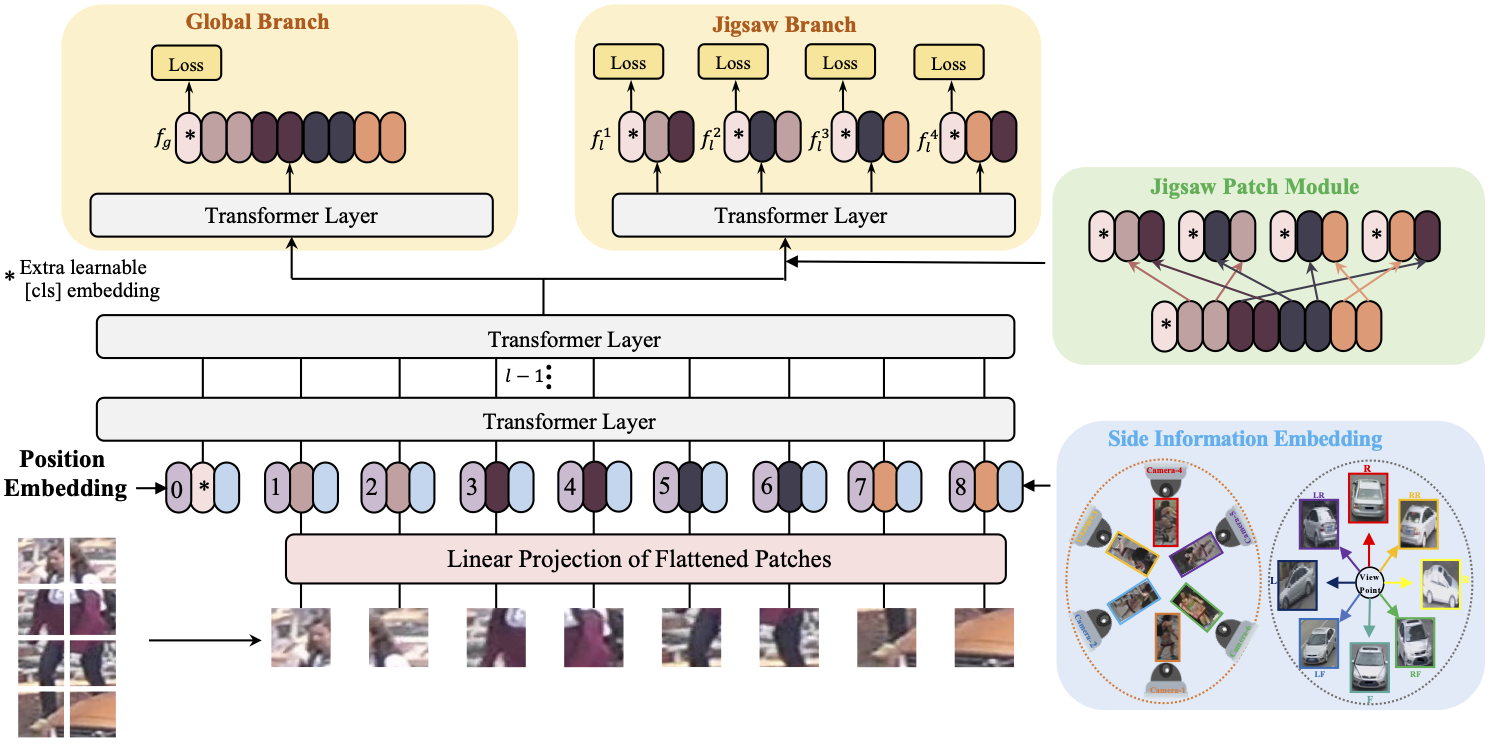
\includegraphics[width=\linewidth,height=.61\textheight,keepaspectratio]{transreid_framework.png}
    \figcaption{Kiến trúc TransReID được dùng làm nền cho các biến thể mở rộng trong đồ án.}
  \end{columns}
  \note{Không đi sâu vào chi tiết cài đặt. Chỉ cần nhấn mạnh các thành phần chính: ViT, SIE, JPM và hai hàm mất mát cơ bản.}
\end{frame}

% 6
\begin{frame}{Hạn chế của biểu diễn cục bộ dựa trên patch}
  \begin{columns}[T,onlytextwidth]
    \column{.54\linewidth}
    \begin{itemize}
      \item Patch cùng vị trí ảnh không luôn tương ứng với cùng vùng cơ thể khi tư thế hoặc crop thay đổi.
      \item Patch nhiễu, bị che khuất hoặc chứa background vẫn có thể ảnh hưởng đến matching.
      \item Biểu diễn cục bộ vì vậy cần thêm tín hiệu bổ trợ ngoài vị trí hình học.
      \item Hai tín hiệu được khai thác trong đồ án là độ tin cậy cục bộ và ngữ nghĩa vùng cơ thể.
    \end{itemize}
    \column{.40\linewidth}
    \begin{block}{Luận điểm chuyển tiếp}
      Vấn đề không chỉ là trích xuất local feature, mà còn là xác định local feature nào đáng tin và local feature đó đang đại diện cho vùng cơ thể nào.
    \end{block}
  \end{columns}
  \note{Đây là slide cầu nối quan trọng giữa baseline và hai hướng mở rộng. Nhấn mạnh hạn chế của patch-level feature khi chỉ dựa trên vị trí hình học.}
\end{frame}

% 7
\begin{frame}{Các hướng mở rộng từ TransReID}
  \small
  \begin{tabularx}{\linewidth}{>{\bfseries}p{.24\linewidth}X X}
    \toprule
    Hướng mở rộng & Tín hiệu bổ sung & Vai trò trong biểu diễn cục bộ \\
    \midrule
    Local Reliability & Mức độ tin cậy của patch token & Giảm ảnh hưởng của vùng nhiễu hoặc bị che khuất. \\
    \addlinespace
    Semantic Alignment & Nhóm semantic của vùng cơ thể & Căn chỉnh local feature theo bộ phận cơ thể tương ứng. \\
    \addlinespace
    Semantic + Reliability & Kết hợp semantic và reliability & Khai thác đồng thời ý nghĩa vùng cơ thể và độ tin cậy cục bộ. \\
    \bottomrule
  \end{tabularx}
  \vspace{.22cm}
  \keymessage{Các hướng mở rộng khai thác những tín hiệu bổ trợ khác nhau trên cùng backbone TransReID.}
  \note{Đây là bản đồ phương pháp của toàn bộ báo cáo. Ba hướng dùng chung backbone nhưng bổ sung các tín hiệu patch-level khác nhau.}
\end{frame}

\section{Phương pháp mở rộng}

% 8
\begin{frame}{Local Reliability: điều chỉnh đóng góp của patch cục bộ}
  \begin{columns}[T,onlytextwidth]
    \column{.50\linewidth}
    \begin{itemize}
      \item Mỗi patch token được gán một mức độ tin cậy.
      \item Patch bị che khuất hoặc chứa nhiễu nền được giảm trọng số.
      \item Reliability score được dùng trong quá trình tổng hợp đặc trưng cục bộ.
      \item Synthetic occlusion cung cấp tín hiệu phụ để học vùng visible và occluded.
    \end{itemize}
    \vspace{.10cm}
    \keymessage{Local Reliability hướng đến việc giảm tác động của các vùng ảnh không đáng tin trong quá trình hình thành embedding cuối.}
    \column{.46\linewidth}
    \centering
    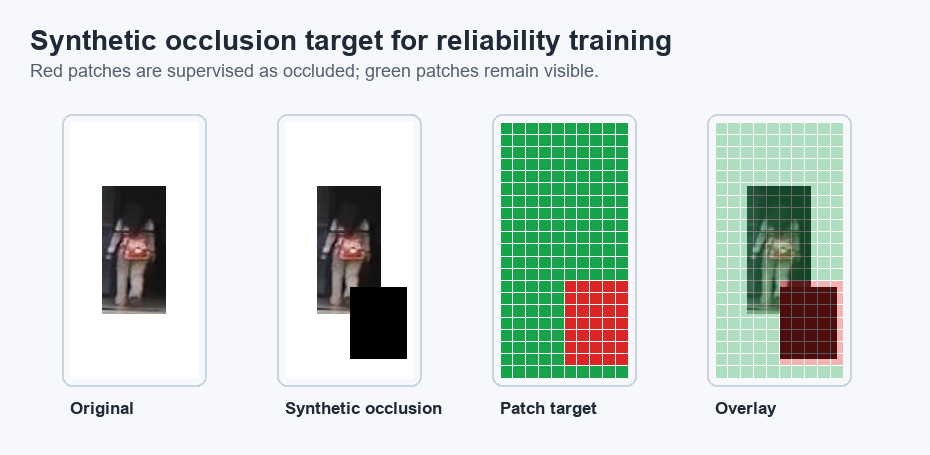
\includegraphics[width=\linewidth,height=.57\textheight,keepaspectratio]{local_synthetic_occlusion_target.png}
    \figcaption{Ví dụ tín hiệu phụ dùng để giám sát vùng bị che khuất trong nhánh Local Reliability.}
  \end{columns}
  \note{Giải thích rằng reliability không thay thế embedding chính, mà điều chỉnh đóng góp của các local token trong bước fusion.}
\end{frame}

% 9
\begin{frame}{Cơ chế tích hợp độ tin cậy cục bộ}
  \centering
  \begin{tikzpicture}[>=Latex,scale=.82,transform shape]
    \tikzstyle{box}=[draw,rounded corners,align=center,minimum width=2.65cm,minimum height=.72cm,fill=SoftGray]
    \node[box,fill=SoftBlue]   (img)   at (0,0.8)   {Ảnh đầu vào};
    \node[box]                 (patch) at (3.1,0.8) {Patch tokens};
    \node[box,fill=SoftOrange] (rel)   at (6.2,0.8) {Reliability\\estimation};
    \node[box]                 (local) at (3.1,-1.0){Local features};
    \node[box,fill=SoftGreen]  (fusion)at (6.2,-1.0){Reliability-aware\\feature fusion};
    \node[box]                 (emb)   at (9.3,-1.0){Re-ID\\embedding};
    \node[box,fill=SoftBlue]   (rank)  at (12.4,-1.0){Ranked\\gallery};
    \draw[->,thick] (img) -- (patch);
    \draw[->,thick] (patch) -- (rel);
    \draw[->,thick] (patch) -- (local);
    \draw[->,thick] (rel) -- (fusion);
    \draw[->,thick] (local) -- (fusion);
    \draw[->,thick] (fusion) -- (emb);
    \draw[->,thick] (emb) -- (rank);
  \end{tikzpicture}
  \vspace{.24cm}
  \begin{itemize}
    \item Đặc trưng cục bộ vẫn được học từ patch token của TransReID.
    \item Reliability score điều chỉnh mức đóng góp của từng patch trước khi tạo embedding cuối.
  \end{itemize}
  \keymessage{Cơ chế này làm cho fusion cục bộ phụ thuộc vào chất lượng quan sát của từng vùng ảnh.}
  \note{Sơ đồ chỉ giữ lại dòng xử lý chính để tránh cảm giác output notebook. Mục tiêu là giải thích logic phương pháp, không đi vào chi tiết triển khai.}
\end{frame}

% 10
\begin{frame}{Trực quan hóa độ tin cậy cục bộ}
  \centering
  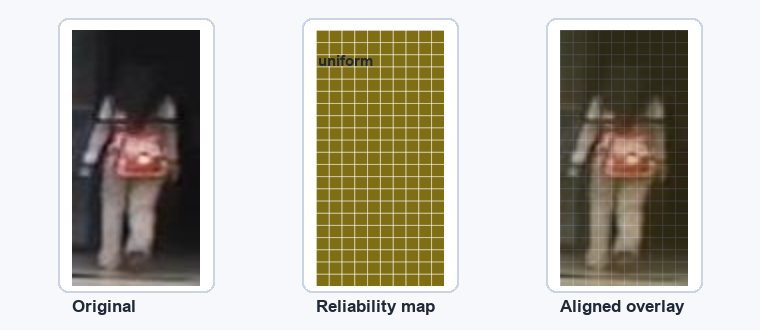
\includegraphics[width=.87\linewidth,height=.48\textheight,keepaspectratio]{local_reliability_heatmap.png}
  \figcaption{Heatmap được ánh xạ lên lưới patch để hỗ trợ diễn giải cơ chế reliability-aware fusion.}
  \vspace{.08cm}
  \begin{itemize}
    \item Heatmap minh họa cách reliability score được ánh xạ lên lưới patch của ảnh đầu vào.
    \item Trực quan hóa này hỗ trợ kiểm tra và diễn giải cơ chế fusion cục bộ.
    \item Đây là phân tích định tính, không thay thế metric định lượng.
  \end{itemize}
  \note{Trình bày thận trọng: heatmap chỉ mang tính giải thích cơ chế, không nên diễn giải quá mạnh như một bằng chứng định lượng.}
\end{frame}

% 11
\begin{frame}{Semantic Alignment: căn chỉnh patch theo vùng cơ thể}
  \begin{columns}[T,onlytextwidth]
    \column{.50\linewidth}
    \begin{itemize}
      \item Human parser phân tách ảnh người thành các vùng cơ thể có ý nghĩa.
      \item Mỗi patch token được gán target semantic theo vùng chiếm ưu thế.
      \item Semantic target giúp local feature gắn với bộ phận cơ thể thay vì chỉ tọa độ ảnh.
      \item Cơ chế này hỗ trợ so sánh các vùng tương ứng giữa nhiều camera.
    \end{itemize}
    \vspace{.10cm}
    \keymessage{Semantic Alignment bổ sung ý nghĩa bộ phận cơ thể cho patch token.}
    \column{.46\linewidth}
    \centering
    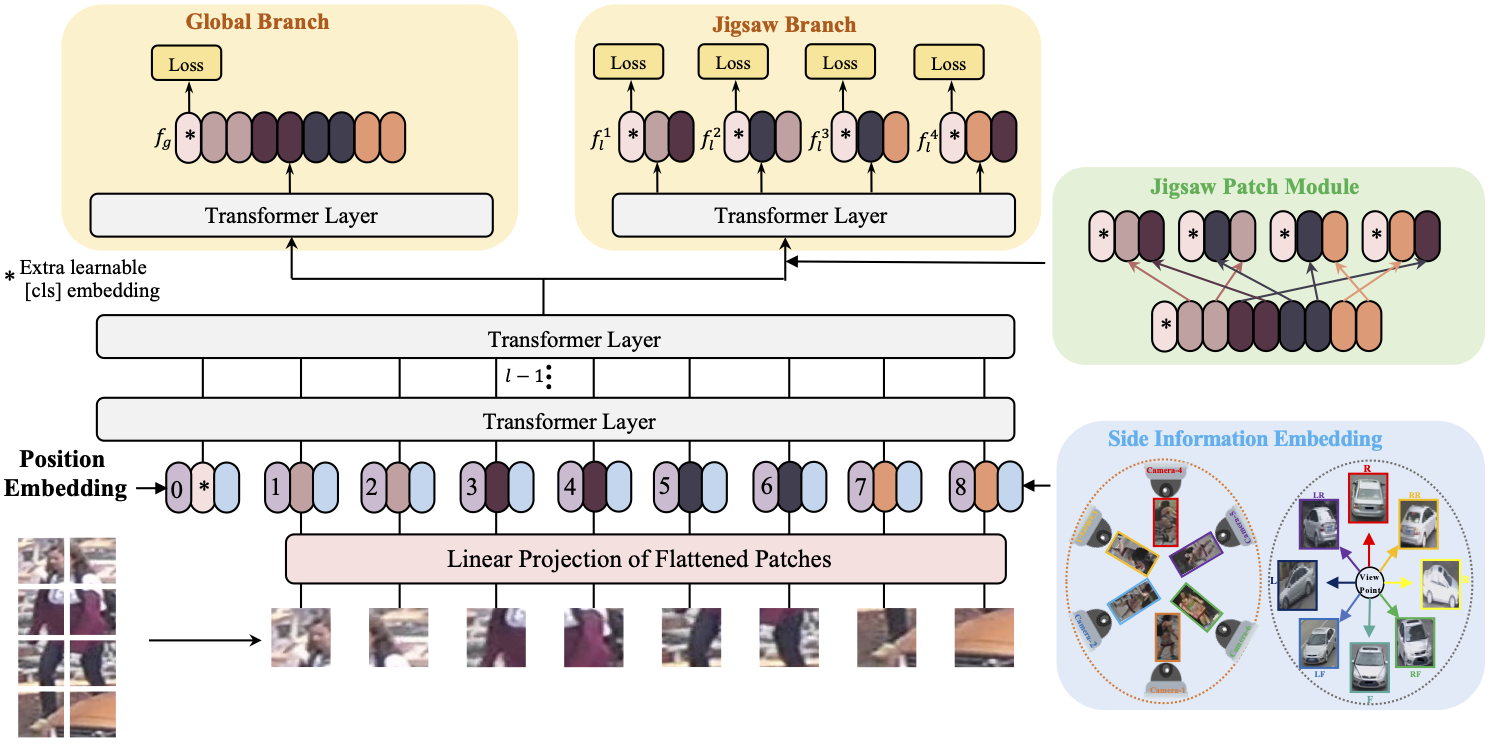
\includegraphics[width=\linewidth,height=.57\textheight,keepaspectratio]{semantic_framework.png}
    \figcaption{Semantic supervision được gắn vào biểu diễn patch-level nhằm hỗ trợ căn chỉnh đặc trưng cục bộ.}
  \end{columns}
  \note{Nhấn mạnh khác biệt với Local Reliability: semantic trả lời patch đang thuộc vùng cơ thể nào, không phải patch đó đáng tin đến đâu.}
\end{frame}

% 12
\begin{frame}{Tạo Semantic Patch Target từ Human Parsing Mask}
  \begin{columns}[T,onlytextwidth]
    \column{.40\linewidth}
    \begin{itemize}
      \item Human parsing mask cung cấp thông tin foreground và vùng cơ thể.
      \item Các nhãn parser được gom thành semantic groups cấp cao.
      \item Transform ảnh và mask được đồng bộ để giữ đúng tương ứng không gian.
      \item Semantic patch target chuyển thông tin mask sang lưới patch của ViT.
    \end{itemize}
    \column{.56\linewidth}
    \centering
    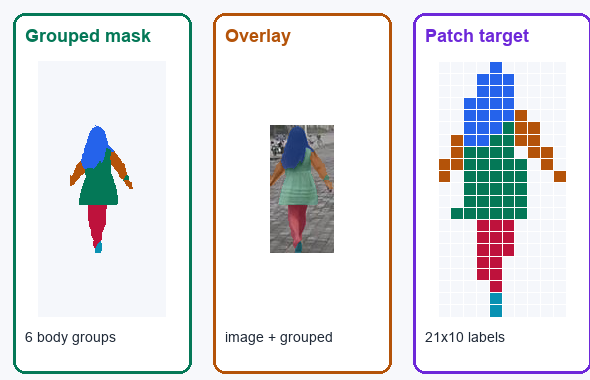
\includegraphics[width=\linewidth,height=.46\textheight,keepaspectratio]{semantic_target_focus.png}
    \vspace{.08cm}
    \figcaption{Mask nhóm vùng cơ thể được chuyển sang patch target để tạo patch-level supervision cho ViT.}
  \end{columns}
  \note{Slide này gộp quy trình tạo target và minh họa patch target để mạch trình bày gọn hơn nhưng vẫn đủ ý.}
\end{frame}

% 13
\begin{frame}{So sánh human parsing mask và mask heuristic}
  \centering
  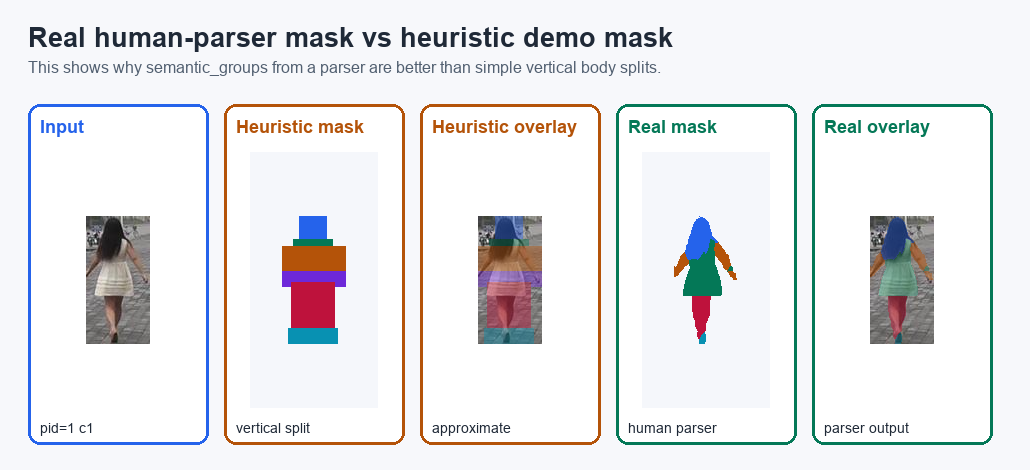
\includegraphics[width=.86\linewidth,height=.60\textheight,keepaspectratio]{semantic_real_vs_heuristic.png}
  \figcaption{Mask heuristic chỉ xấp xỉ theo hình học, trong khi human parsing mask bám sát silhouette, trang phục và tư thế hơn.}
  \vspace{.05cm}
  \begin{itemize}
    \item Mask heuristic đơn giản nhưng thiếu thông tin về hình dạng và tư thế người.
    \item Human parsing mask phù hợp hơn để tạo semantic supervision cho patch token.
  \end{itemize}
  \note{Giữ giọng điệu học thuật trung tính: heuristic có ưu điểm về đơn giản, nhưng parser mask tốt hơn cho mục tiêu semantic alignment.}
\end{frame}

% 14
\begin{frame}{Tính nhất quán semantic giữa các góc nhìn camera}
  \centering
  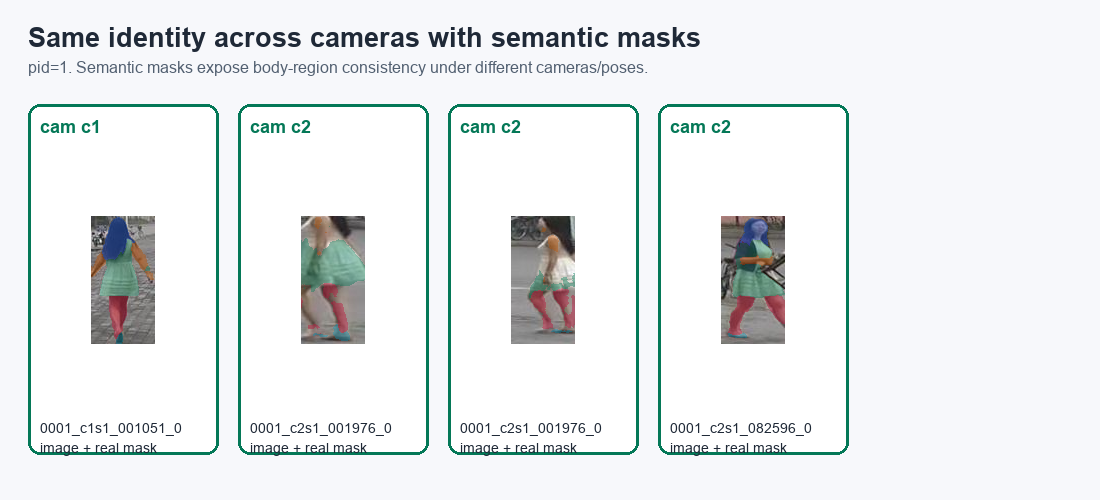
\includegraphics[width=.74\linewidth,height=.44\textheight,keepaspectratio]{semantic_same_identity.png}
  \figcaption{Semantic mask tạo tham chiếu theo bộ phận cơ thể của cùng một ID qua nhiều camera.}
  \vspace{.02cm}
  \begin{itemize}
    \item Cùng một ID có thể xuất hiện dưới nhiều tư thế, crop và camera khác nhau.
    \item Semantic mask tạo điểm tham chiếu theo vùng cơ thể thay vì theo tọa độ ảnh tuyệt đối.
    \item Điều này hỗ trợ so sánh local feature giữa các ảnh có biến thiên quan sát lớn.
  \end{itemize}
  \vspace{.02cm}
  \keymessage{Semantic Alignment hỗ trợ so sánh các vùng cơ thể tương ứng thay vì phụ thuộc vào tọa độ ảnh tuyệt đối.}
  \note{Nêu ví dụ trực quan: torso hoặc legs có thể nằm ở vị trí ảnh khác nhau, nhưng semantic mask vẫn tạo khung tham chiếu theo bộ phận cơ thể.}
\end{frame}

% 15
\begin{frame}{Kết hợp căn chỉnh semantic và độ tin cậy cục bộ}
  \small
  \begin{columns}[T,onlytextwidth]
    \column{.47\linewidth}
    \begin{itemize}
      \item Semantic Alignment xác định ý nghĩa vùng cơ thể của patch.
      \item Local Reliability ước lượng mức độ tin cậy của patch.
      \item Hai tín hiệu này bổ sung nhau trong biểu diễn cục bộ: semantic xác định vùng có ý nghĩa, còn reliability giảm ảnh hưởng của vùng kém tin cậy.
      \item Hướng kết hợp khai thác đồng thời hai tín hiệu này trong quá trình tổng hợp đặc trưng.
      \item Mục tiêu là tăng chất lượng embedding khi có thay đổi tư thế, nhiễu nền hoặc che khuất.
    \end{itemize}
    \column{.49\linewidth}
    \centering
    \begin{tikzpicture}[node distance=.44cm,>=Latex,scale=.78,transform shape]
      \tikzstyle{box}=[draw,rounded corners,align=center,minimum width=2.50cm,minimum height=.62cm,fill=SoftGray]
      \node[box,fill=SoftBlue] (img) {Ảnh đầu vào};
      \node[box,below=of img] (vit) {Patch tokens};
      \node[box,fill=SoftGreen,below left=.55cm and .55cm of vit] (sem) {Semantic\\groups};
      \node[box,fill=SoftOrange,below right=.55cm and .55cm of vit] (rel) {Reliability\\scores};
      \node[box,below=1.5cm of vit] (fusion) {Structured\\feature fusion};
      \node[box,fill=SoftBlue,below=of fusion] (emb) {Re-ID\\embedding};
      \node[box,fill=SoftGreen,below=of emb] (rank) {Ranking};
      \draw[->,thick] (img) -- (vit);
      \draw[->,thick] (vit) -- (sem);
      \draw[->,thick] (vit) -- (rel);
      \draw[->,thick] (sem) -- (fusion);
      \draw[->,thick] (rel) -- (fusion);
      \draw[->,thick] (fusion) -- (emb);
      \draw[->,thick] (emb) -- (rank);
    \end{tikzpicture}
  \end{columns}
  \vspace{.08cm}
  \keymessage{Hướng kết hợp nhằm giữ lại các vùng vừa có ý nghĩa semantic, vừa đáng tin cậy cho matching.}
  \note{Nhấn mạnh đây là giả thuyết phương pháp dựa trên tính bổ trợ của hai tín hiệu, không diễn giải như một giải pháp triệt để cho mọi tình huống.}
\end{frame}

\section{Thiết lập thực nghiệm}

% 16
\begin{frame}{Thiết lập thực nghiệm trên Market-1501}
  \small
  \begin{itemize}
    \item Market-1501 gồm ảnh người từ nhiều camera, phù hợp để đánh giá khả năng truy hồi danh tính liên camera.
    \item Tất cả biến thể được đánh giá trên cùng backbone, cùng tập dữ liệu và cùng metric để đảm bảo so sánh nhất quán.
  \end{itemize}
  \vspace{.08cm}
  \begin{tabularx}{\linewidth}{>{\bfseries}p{.25\linewidth}X X}
    \toprule
    Biến thể & Mục đích đánh giá & Vai trò trong so sánh \\
    \midrule
    TransReID baseline & Mô hình nền dựa trên ViT & Mốc so sánh gốc. \\
    Semantic Alignment & Giám sát semantic cho patch token & Đánh giá tác động của thông tin vùng cơ thể. \\
    Local Reliability & Điều chỉnh đóng góp của patch cục bộ & Đánh giá tác động của độ tin cậy patch. \\
    Semantic + Reliability & Kết hợp hai tín hiệu bổ trợ & Đánh giá khả năng bổ sung lẫn nhau. \\
    \bottomrule
  \end{tabularx}
  \vspace{.18cm}
  \begin{block}{Protocol đánh giá}
    Dataset Market-1501; các mô hình dùng cùng backbone và protocol đánh giá; metric gồm mAP, CMC Rank-1/Rank-5/Rank-10 và latency.
  \end{block}
  \note{Không đưa đường dẫn, checkpoint hay tên script lên slide chính. Trọng tâm là tính công bằng của protocol giữa các biến thể.}
\end{frame}

\section{Kết quả và phân tích}

% 17
\begin{frame}{Kết quả định lượng trên Market-1501}
  \centering
  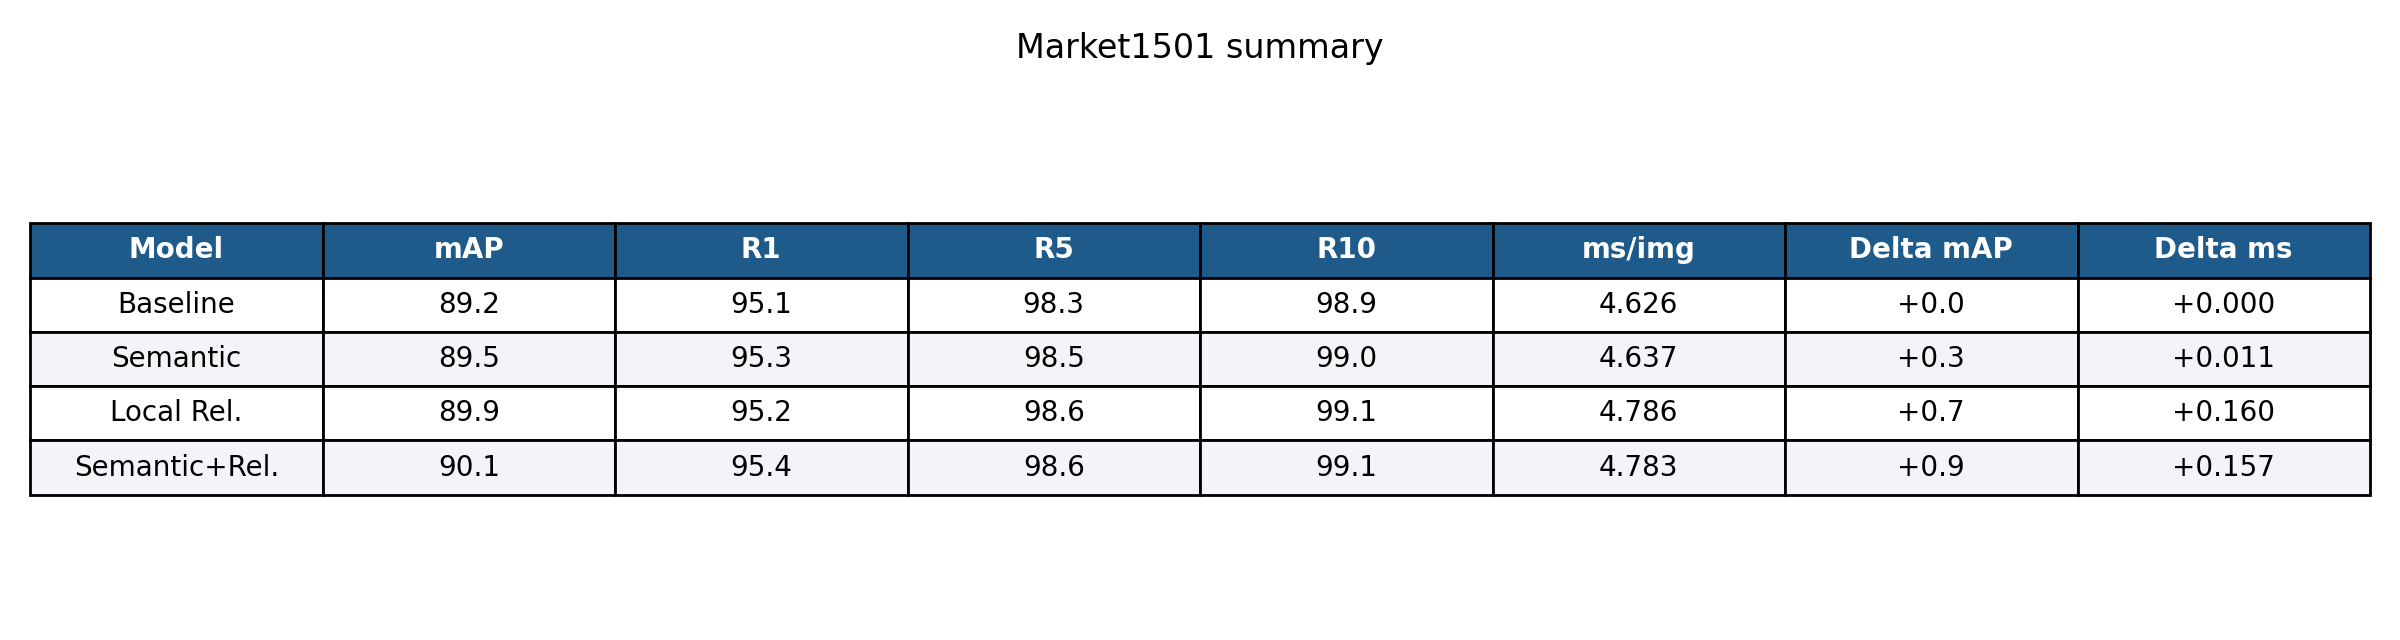
\includegraphics[width=.95\linewidth,height=.66\textheight,keepaspectratio]{eval_summary_table.png}
  \figcaption{Bảng tổng hợp cho thấy các tín hiệu bổ trợ ở mức patch token có xu hướng cải thiện chất lượng retrieval so với baseline.}
  \vspace{.08cm}
  \keymessage{Semantic + Reliability đạt mAP và Rank-1 cao nhất trong bộ thử nghiệm, nhưng chênh lệch Rank-1 tương đối nhỏ.}
  \note{Nhấn mạnh kết quả cao nhất trong phạm vi bộ thử nghiệm hiện tại, không dùng ngôn ngữ overclaim.}
\end{frame}

% 18
\begin{frame}{So sánh mAP và CMC Rank-k}
  \centering
  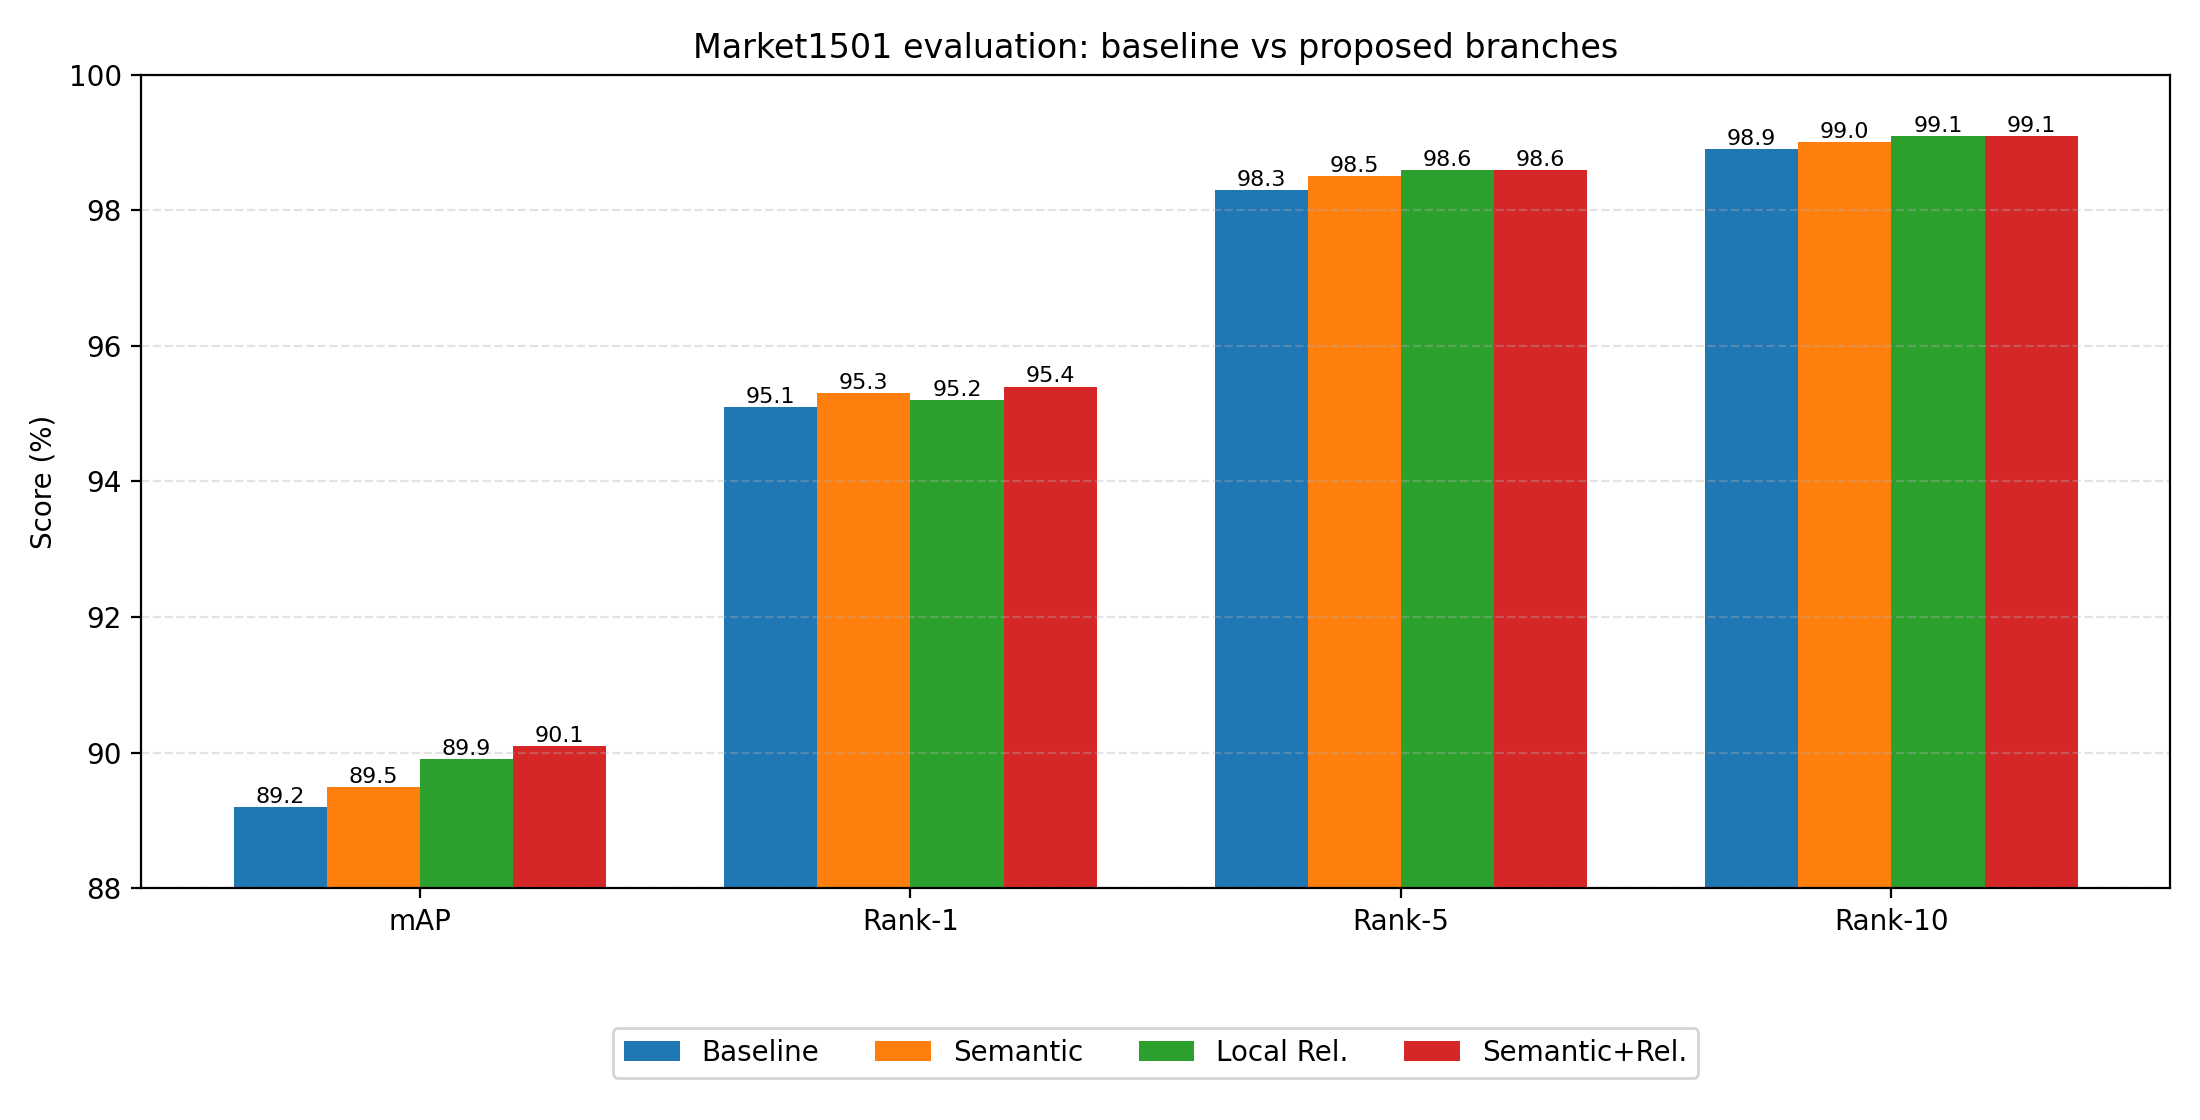
\includegraphics[width=.90\linewidth,height=.61\textheight,keepaspectratio]{eval_metrics_grouped_bar.png}
  \figcaption{Mức tăng mAP rõ hơn CMC Rank-k, cho thấy chất lượng sắp xếp toàn bộ gallery được cải thiện rõ hơn so với chỉ số top-1.}
  \vspace{.05cm}
  \keymessage{Các hướng mở rộng đều cho thấy xu hướng cải thiện so với baseline trên Market-1501.}
  \note{Giải thích ngắn rằng mAP phản ánh toàn bộ ranking, nên nhạy hơn Rank-1 khi mức cải thiện tập trung ở chất lượng sắp xếp chung.}
\end{frame}

% 19
\begin{frame}{Phân tích kết quả định lượng}
  \begin{columns}[T,onlytextwidth]
    \column{.48\linewidth}
    \begin{itemize}
      \item Semantic + Reliability đạt mAP và Rank-1 cao nhất trong bộ thử nghiệm.
      \item Local Reliability cải thiện mAP rõ rệt hơn so với Rank-1.
      \item mAP phản ánh chất lượng xếp hạng toàn bộ gallery, trong khi CMC Rank-k tập trung vào vị trí xuất hiện của ảnh đúng trong top-k.
      \item mAP nhạy hơn Rank-1 vì phản ánh toàn bộ danh sách truy hồi.
      \item Kết quả hiện tại ủng hộ hướng mở rộng patch-level nhưng chưa đủ để kết luận tổng quát.
    \end{itemize}
    \column{.48\linewidth}
    \centering
    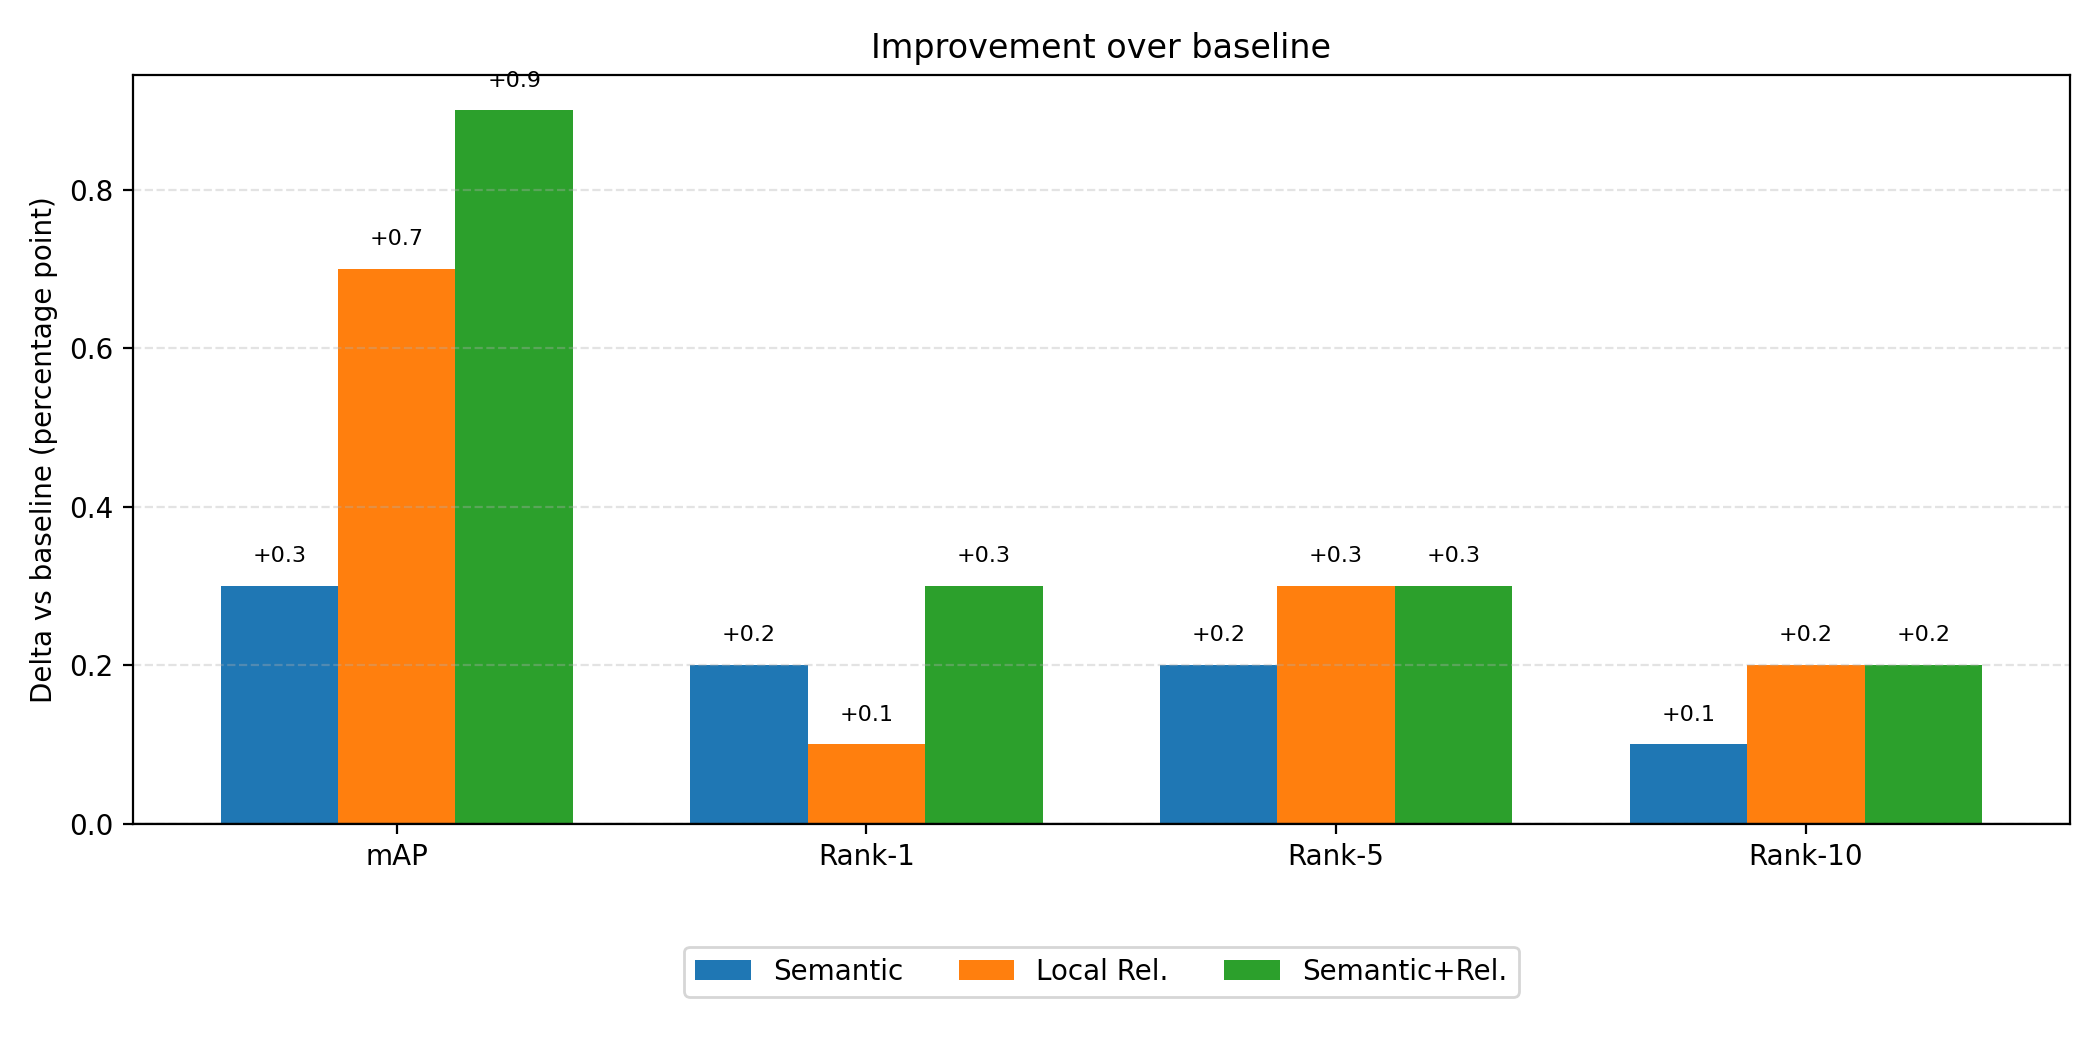
\includegraphics[width=\linewidth,height=.48\textheight,keepaspectratio]{eval_delta_vs_baseline.png}
    \figcaption{Mức thay đổi theo từng metric khi so với baseline.}
  \end{columns}
  \note{Đây là slide diễn giải số liệu. Cách nói cần thận trọng, đặc biệt với Rank-1 vì baseline đã khá mạnh.}
\end{frame}

% 20
\begin{frame}{Quá trình hội tụ trong huấn luyện}
  \begin{columns}[T,onlytextwidth]
    \column{.58\linewidth}
    \centering
    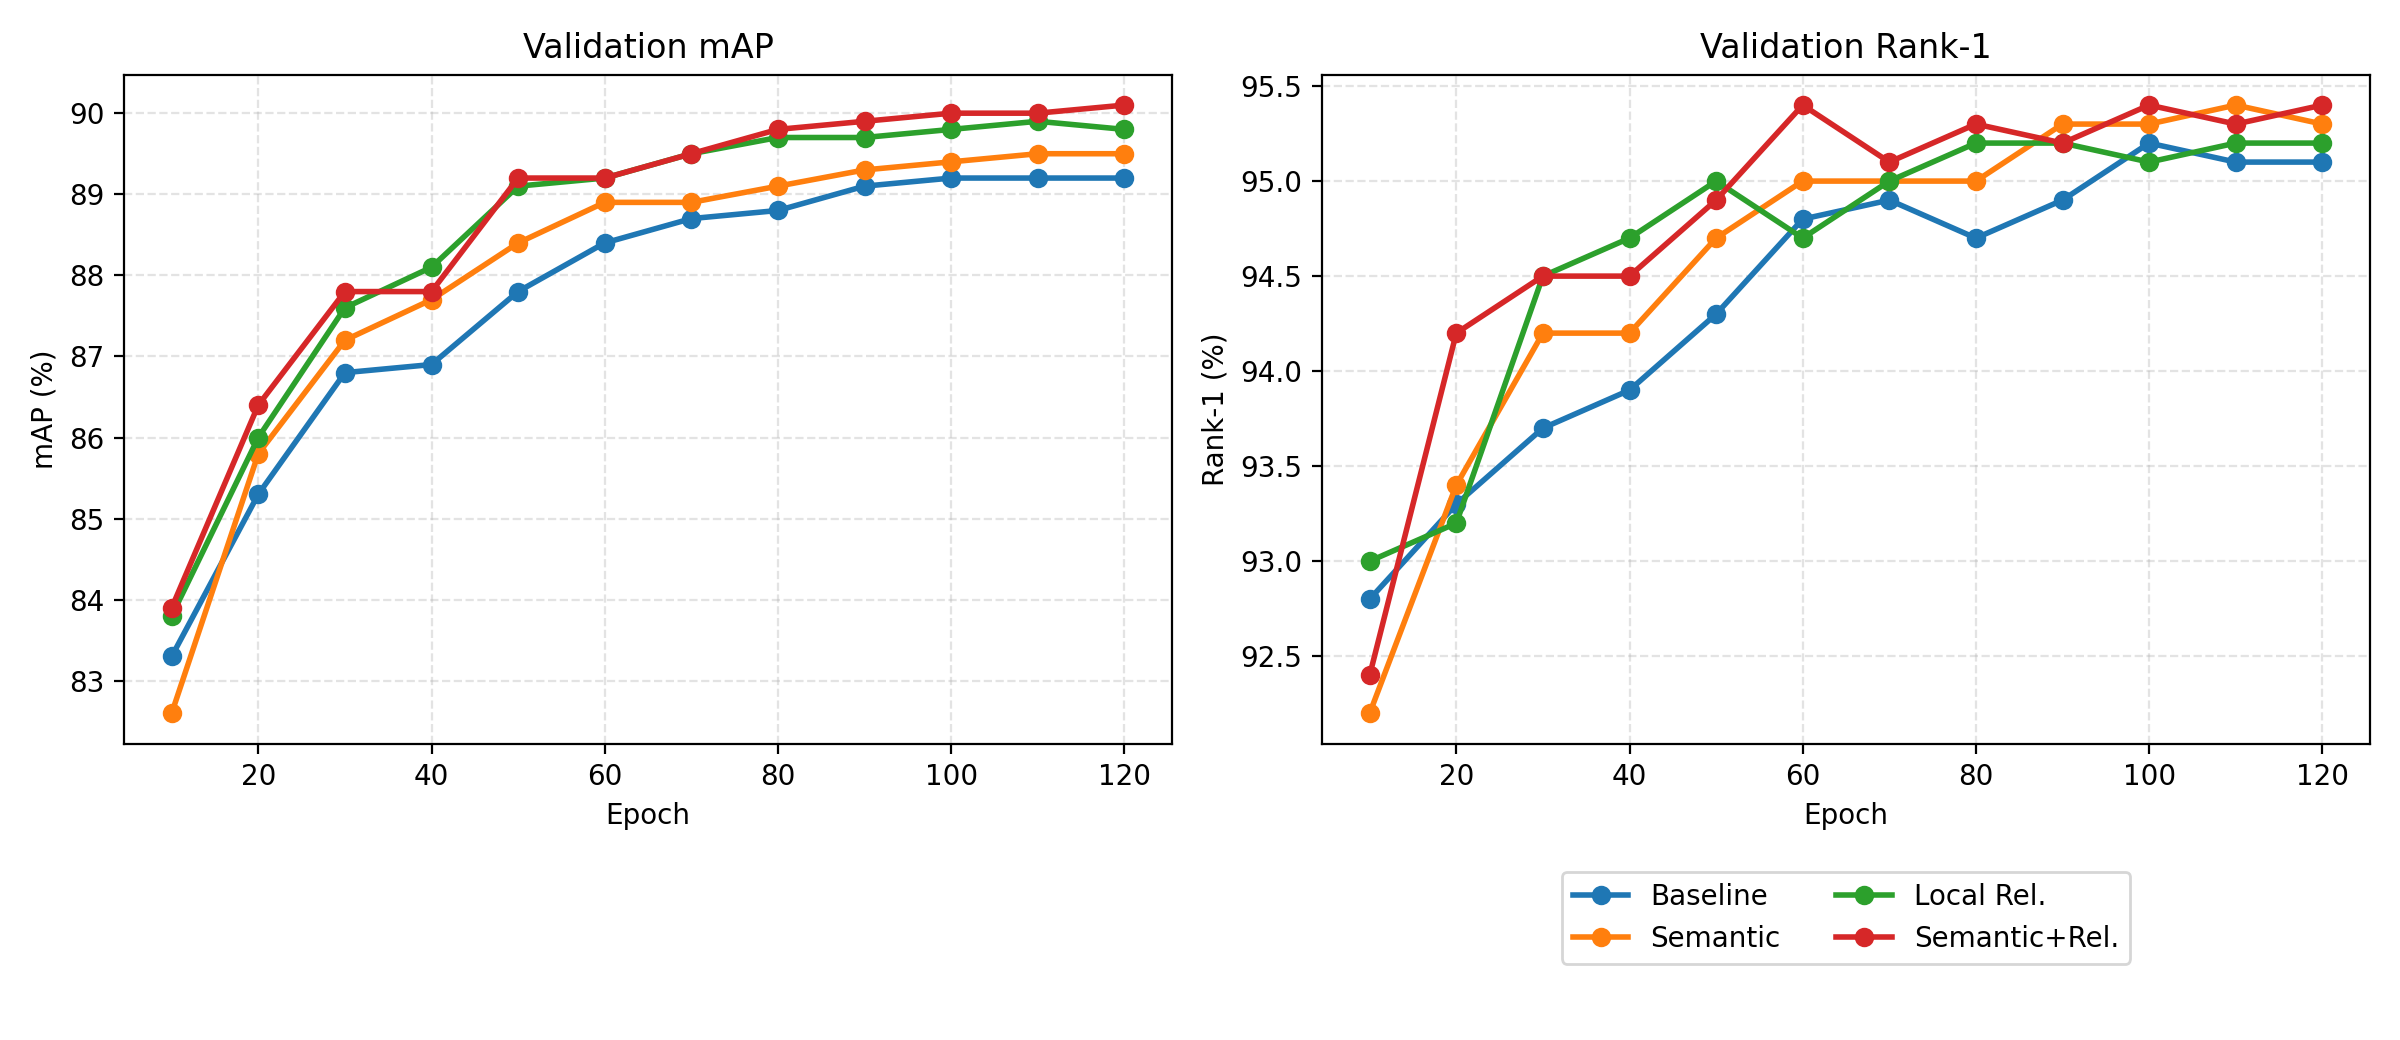
\includegraphics[width=\linewidth,height=.60\textheight,keepaspectratio]{eval_validation_map_rank1_curves.png}
    \figcaption{Validation mAP và Rank-1 theo epoch của các biến thể.}
    \column{.38\linewidth}
    \begin{itemize}
      \item Các mô hình hội tụ tương đối ổn định.
      \item Khoảng cách giữa các biến thể không quá lớn.
      \item Checkpoint tốt nhất của hướng kết hợp nhỉnh hơn nhẹ ở mAP và Rank-1.
    \end{itemize}
  \end{columns}
  \note{Giữ cách diễn giải tiết chế: đồ thị hỗ trợ quan sát xu hướng hội tụ, không nhằm khẳng định chênh lệch lớn giữa các mô hình.}
\end{frame}

% 21
\begin{frame}{So sánh định tính trên cùng truy vấn}
  \begin{columns}[T,onlytextwidth]
    \column{.58\linewidth}
    \centering
    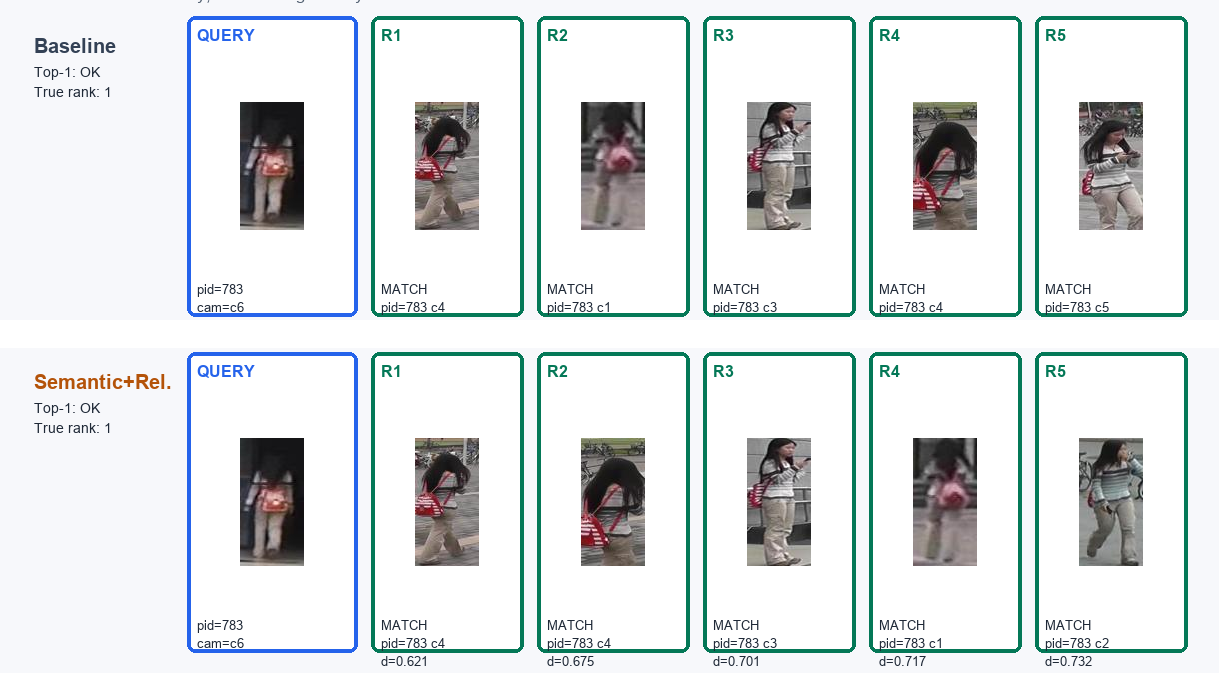
\includegraphics[width=\linewidth,height=.64\textheight,keepaspectratio]{multi_model_same_query_topk_focus.png}
    \figcaption{Hình minh họa xu hướng thay đổi thứ hạng của ảnh đúng và ảnh sai trên cùng truy vấn.}
    \column{.38\linewidth}
    \begin{itemize}
      \item Cùng một query và gallery được chạy qua các biến thể để so sánh trực tiếp.
      \item Khác biệt chủ yếu nằm ở thứ hạng của ảnh đúng trong danh sách Top-K.
      \item Hình dùng để minh họa xu hướng ranking, không nhằm thay thế đánh giá định lượng.
    \end{itemize}
    \vspace{.12cm}
    \keymessage{Sự khác biệt giữa các mô hình thể hiện rõ hơn ở chất lượng sắp xếp hơn là chỉ ở nhãn đúng hoặc sai Top-1.}
  \end{columns}
  \note{Không cần đọc toàn bộ từng ô. Chỉ hướng người xem quan sát vị trí của ảnh đúng và sự thay đổi thứ hạng giữa các mô hình.}
\end{frame}

% 22
\begin{frame}{Phân tích lỗi trong bài toán truy hồi theo ranking}
  \begin{columns}[T,onlytextwidth]
    \column{.48\linewidth}
    \centering
    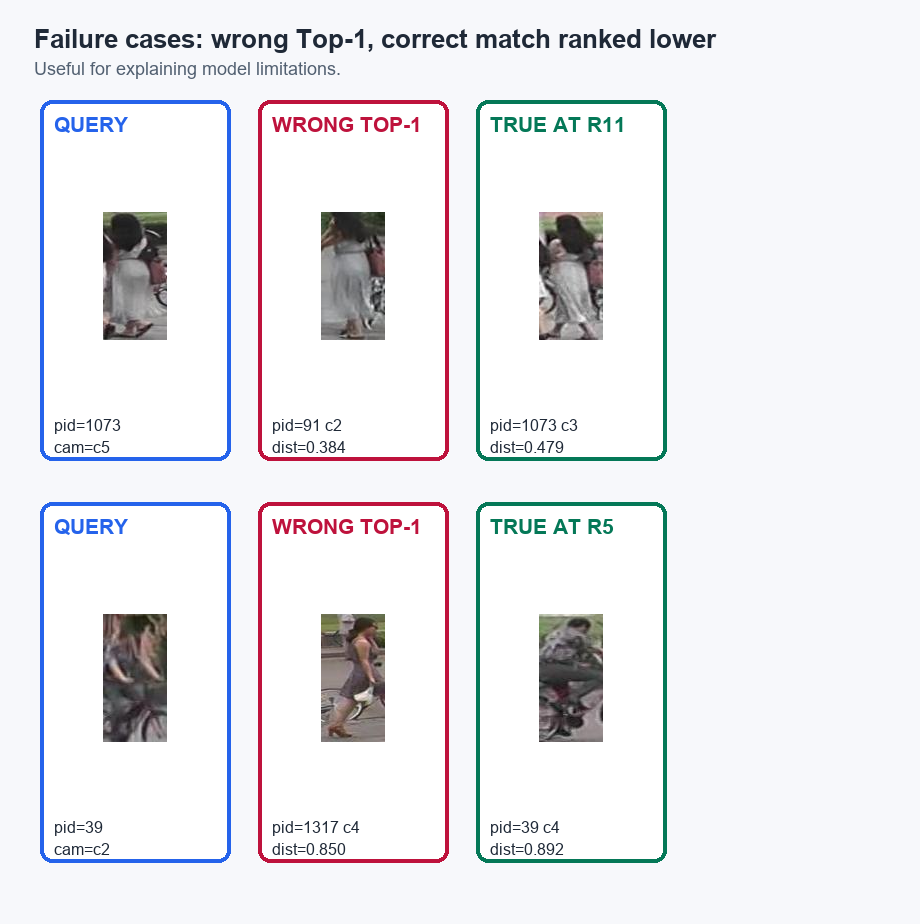
\includegraphics[width=\linewidth,height=.60\textheight,keepaspectratio]{local_failure_cases.png}
    \figcaption{Failure cases minh họa giới hạn của mô hình trong các tình huống truy hồi khó.}
    \column{.48\linewidth}
    \begin{itemize}
      \item Re-ID không chỉ đánh giá đúng hoặc sai tại Top-1 mà cần xem toàn bộ thứ hạng.
      \item Ảnh đúng có thể bị đẩy xuống rank thấp do hard negatives, pose tương tự, trang phục giống, background, crop hoặc occlusion.
      \item Failure cases định hướng phân tích sâu hơn theo camera ID, occlusion và pose.
    \end{itemize}
    \vspace{.12cm}
    \keymessage{Rank-1 cao không đồng nghĩa mô hình đã xử lý đầy đủ mọi tình huống Re-ID.}
  \end{columns}
  \note{Gộp failure cases với ý nghĩa của phân tích lỗi để phần định tính gọn hơn và gắn trực tiếp với bản chất ranking của bài toán.}
\end{frame}

% 23
\begin{frame}{Đánh đổi giữa hiệu quả truy hồi và chi phí suy luận}
  \begin{columns}[T,onlytextwidth]
    \column{.56\linewidth}
    \centering
    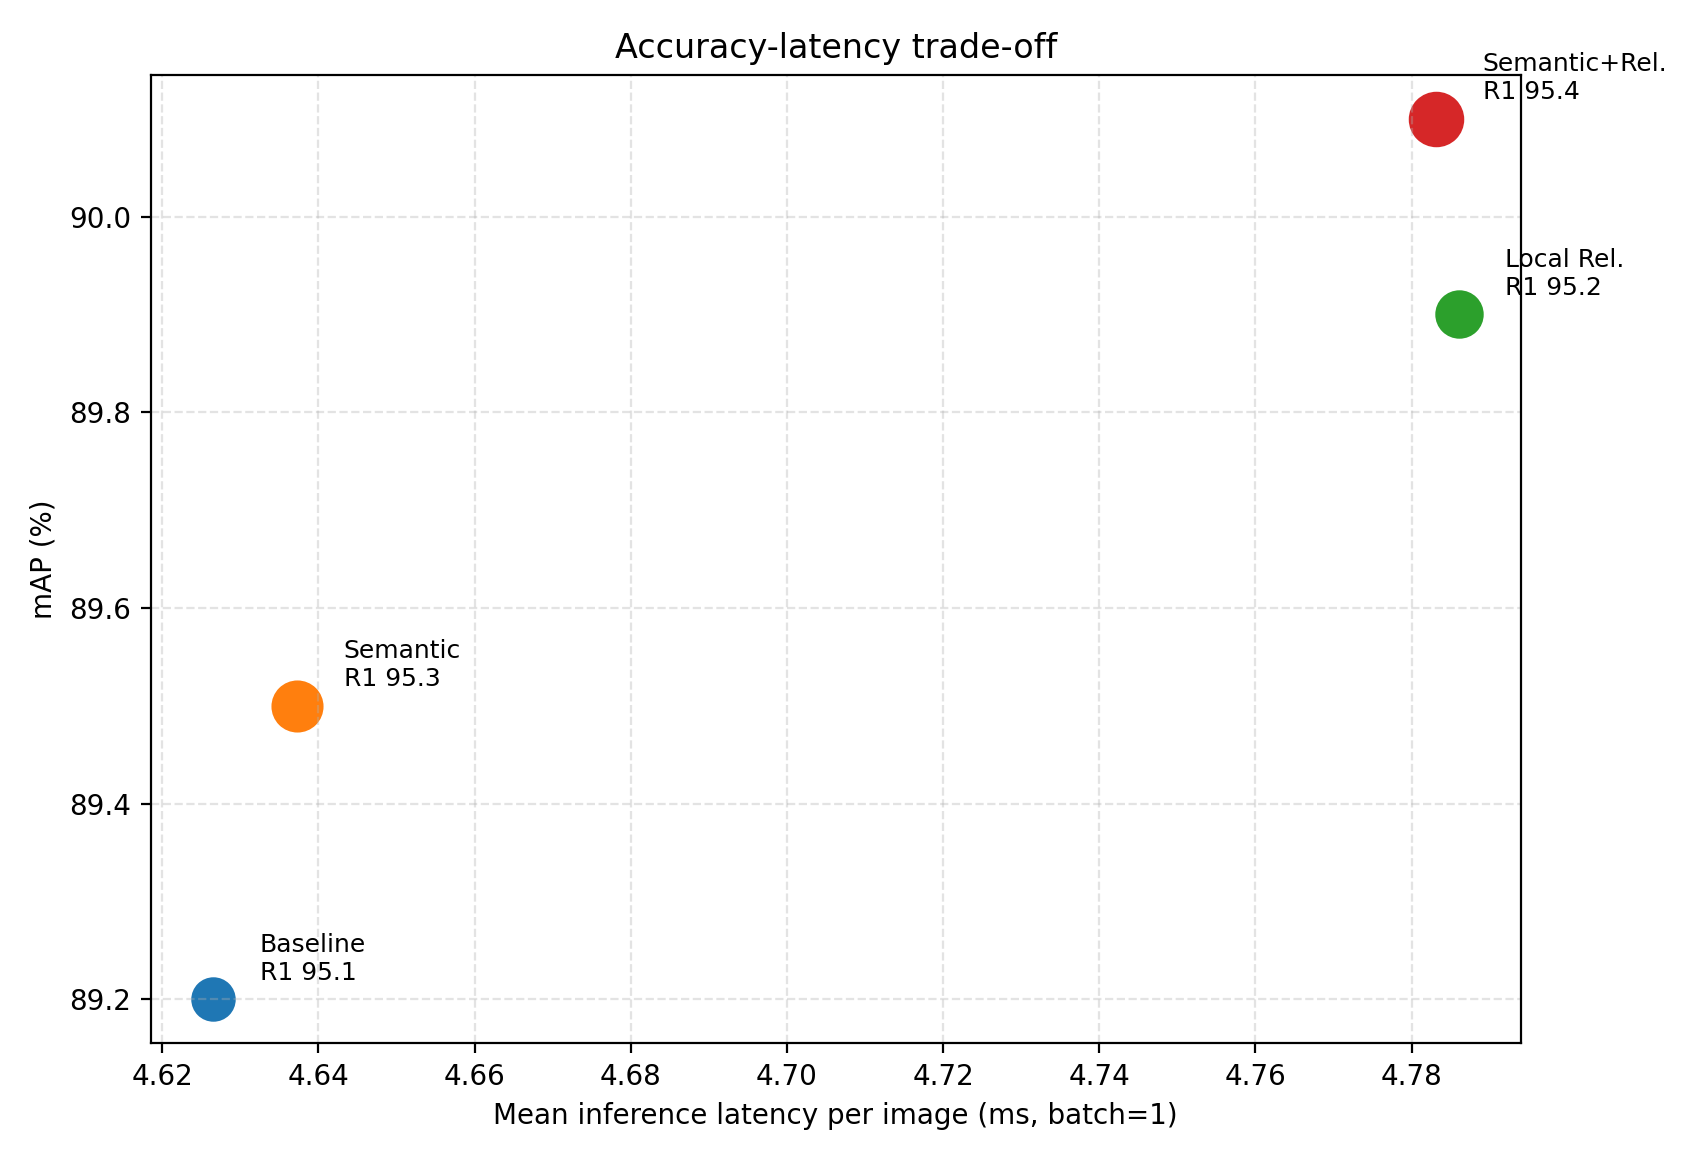
\includegraphics[width=\linewidth,height=.60\textheight,keepaspectratio]{eval_accuracy_latency_tradeoff.png}
    \figcaption{Quan hệ giữa mAP và latency trung bình trong thí nghiệm hiện tại.}
    \column{.40\linewidth}
    \begin{itemize}
      \item Semantic Alignment có latency gần baseline.
      \item Local Reliability và Semantic + Reliability tăng nhẹ chi phí suy luận.
      \item Hướng kết hợp đạt chất lượng truy hồi cao nhất trong bộ thử nghiệm.
      \item Mức tăng latency vẫn nhỏ trong thiết lập đo hiện tại.
      \item Cần đo lại trong môi trường ổn định hơn nếu hướng đến triển khai thực tế.
    \end{itemize}
  \end{columns}
  \note{Gộp phần biểu đồ và tổng hợp trade-off vào một slide để rút gọn deck mà vẫn giữ được ý chính về hiệu quả và overhead.}
\end{frame}

\section{Tổng kết}

% 24
\begin{frame}{Đóng góp chính của đồ án}
  \begin{itemize}
    \item Thiết lập pipeline đánh giá Person Re-ID dựa trên TransReID.
    \item Huấn luyện và đánh giá bốn biến thể trên cùng protocol thực nghiệm.
    \item Xây dựng trực quan hóa phục vụ phân tích retrieval, semantic mask, reliability và failure cases.
    \item Tổng hợp đánh giá định lượng, định tính và chi phí suy luận.
  \end{itemize}
  \note{Nhấn mạnh đóng góp ở mức thực nghiệm và phân tích, tránh kể lại các file hoặc script đã tạo.}
\end{frame}

% 25
\begin{frame}{Hạn chế hiện tại}
  \begin{itemize}
    \item Thực nghiệm hiện mới tập trung trên Market-1501.
    \item Mức tăng Rank-1 còn nhỏ do baseline đã mạnh.
    \item Semantic supervision phụ thuộc vào chất lượng của human parser.
    \item Chưa có ablation đủ chi tiết cho từng loss và từng thành phần fusion.
  \end{itemize}
  \vspace{.16cm}
  \keymessage{Kết quả hiện tại cho thấy xu hướng tích cực trên Market-1501, nhưng chưa đủ để khẳng định tính tổng quát trên các bối cảnh Re-ID có occlusion nặng.}
  \note{Giữ thái độ học thuật trung thực: có xu hướng tích cực nhưng chưa đủ để khẳng định kết luận rộng hơn.}
\end{frame}

% 26
\begin{frame}{Định hướng phát triển tiếp theo}
  \begin{itemize}
    \item Đánh giá trên Occluded-DukeMTMC hoặc các tập có nhiều che khuất.
    \item Ablation từng thành phần: semantic supervision, reliability loss và fusion strategy.
    \item Phân tích lỗi theo camera ID, pose, occlusion và background.
    \item Tối ưu inference nếu hướng đến triển khai thực tế.
  \end{itemize}
  \note{Các bước tiếp theo được sắp theo mức độ ưu tiên: mở rộng dataset, làm ablation, phân tích lỗi sâu hơn rồi tối ưu suy luận.}
\end{frame}

% 27
\begin{frame}{Kết luận}
  \begin{columns}[T,onlytextwidth]
    \column{.48\linewidth}
    \begin{block}{Local Reliability}
      Giảm ảnh hưởng của patch nhiễu hoặc bị che khuất trong quá trình hình thành embedding cuối.
    \end{block}
    \begin{block}{Semantic Alignment}
      Đưa thông tin vùng cơ thể vào biểu diễn patch-level thay vì chỉ dựa trên vị trí hình học.
    \end{block}
    \column{.48\linewidth}
    \begin{block}{Hướng kết hợp}
      Đạt kết quả cao nhất trong bộ thử nghiệm Market-1501 và gợi ý tính bổ trợ giữa hai tín hiệu.
    \end{block}
    \begin{block}{Thông điệp}
      Biểu diễn cục bộ có cấu trúc là hướng tiềm năng để cải thiện Person Re-ID trên nền TransReID.
    \end{block}
  \end{columns}
  \vspace{.16cm}
  \centering
  \Large Cảm ơn thầy/cô và các bạn đã lắng nghe
  \note{Kết lại bằng ba ý chính: Local Reliability xử lý độ tin cậy, Semantic Alignment xử lý ý nghĩa vùng cơ thể, và hướng kết hợp cho kết quả tốt nhất trong phạm vi thực nghiệm hiện tại.}
\end{frame}

\end{document}
